\documentclass[a4paper,12pt]{article}
\parindent 1cm
\parskip 1mm
\usepackage{amsmath}
\usepackage[dvips]{epsfig}

\begin{document}

\begin{center}

{\Large\bf CN 530 - Computational Models of Vision}

\bigskip

{\large\bf Assignment \# 3}
\vspace{0.1mm}

\end{center}

{\bf Abstract}
\smallskip

The goal of this assignment is to replicate the one-dimensional data produced by the model outlined in the 1988 paper by Grossberg and Mingolla $Neural dynamics of 1-D and 2-D brightness perception: A unified model of classical and recent phenomena$. I have constructed the six layer model outlined therein using C and supplied it with several input patterns. Each layer processes the input of the previous in order to produce the final result, and we will observe the output of several layers and try to understand how their coming together yielded the final result. 
\smallskip

Two methods of simulating the diffusion process outlined in the final stage as well as their convergence properties will be discussed, and we will also compare this model to a model outlined by Craft et. al dealing with Border Ownership. 
\bigskip

{\bf Item 1}
\smallskip

The model outlined in the aforementioned paper consists of six layers each consiting of a 1-dimensional receptive field of 100 cells. The first layer recieves the input and the second performs a convolution with a difference-of-Gaussians (DoG) kernel. Layers 3 through 5 determine the direction of edges detected by Layer 2 and use this information to generate boundaries within the input space. In the final layer the brightness data from Layer two is allowed to diffuse throughout the image; this diffusion process is halted by the presence of boundaries that were detected in layer 5. 
\smallskip

The goal of this is to replicate the process of filling in, whereby object features spread throughout the interior of the space they occupy within an image. This model was implemented by me in C using the following $\verbatim{struct}$ to describe a layer:

\begin{verbatim}
struct Layer{
   float * input;
   float * output;
   FILE * data;
}
\end{verbatim} 

The input of each layer is always the output of the previous layer, and accordingly every layer's output goes into another's input. The data file is used to output the results of each layer. In the first five layers solutions were computed at equilibirium, though in the future I would like to explore the temporal dynamics of each layer in a real time simulation. 
\smallskip

To test the model a basic bar input pattern was presented that took on a value of 10 between cells 20 and 80 and 0 everywhere else. In the plot below we see this input pattern as well as the results from layers 2 (DoG Kernel Convolution) and 5 (border detection). 

\begin{center}
  \begin{figure}[h!]
    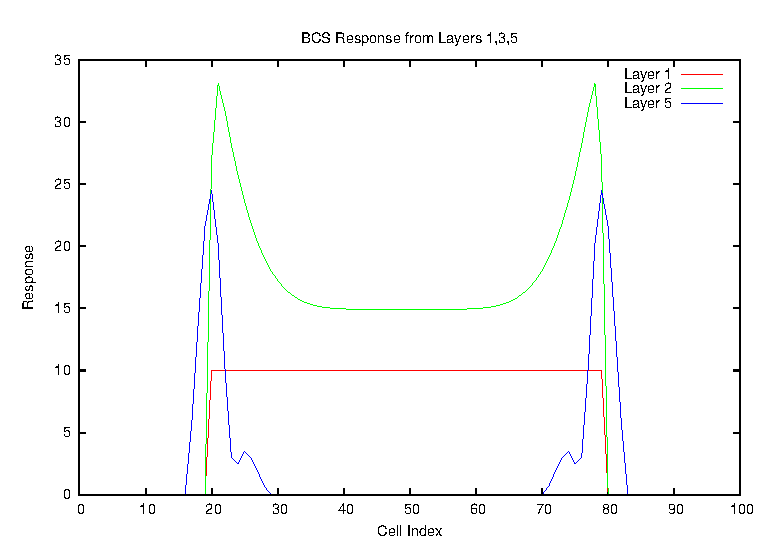
\epsfig{file=fig1.eps,width=15cm,height=11cm}
    \caption{\label{pict1}Response of BCS to Bar Input}
  \end{figure}
\end{center}

Notice the large differences in output scale here. I tried several parameter variations but was unable to get Layers 2 and 5 to appear on the same relative scale, though I suppose this is not important. However, when computing Layer 6 I noticed that its response was significantly lower than the rest. This does seem to follow the data I set out to replicate, but I still thought it strange. The figure below was produced from the same bar input, and the diffusion was solved for using the relaxation method. 

\begin{center}
  \begin{figure}[h!]
    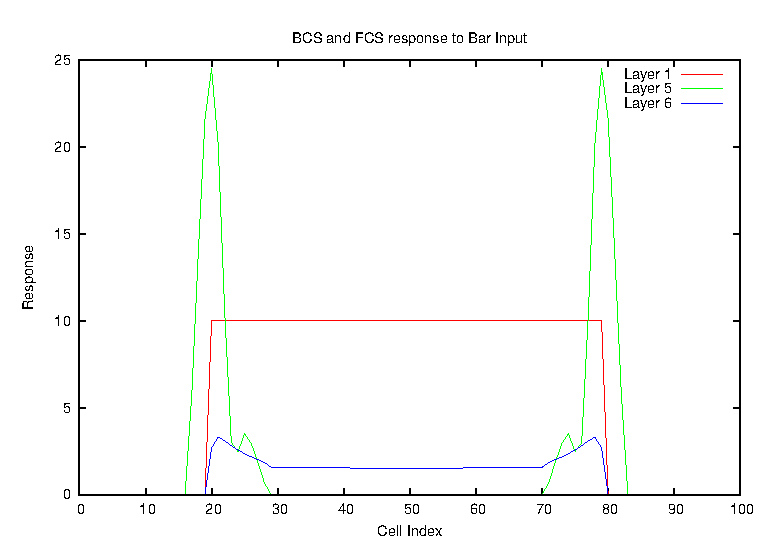
\epsfig{file=fig2.eps,width=15cm,height=11cm}
    \caption{\label{pict1}BCS and FCS output}
  \end{figure}
\end{center}

It seems to me that we don't really gain a whole lot by computing the FCS. I may have made an error, but the result I get appears to be a damped version of Layer 2's reponse. By varying parameters I confirmed that I could control the spread of output within the enclosed region, but the results were often quite boring. It seems to me that if anything information is lost during the generation of the FCS. 
\smallskip

In terms of data replication, I had trouble making my model respond correctly to the COCE. I don't think I replicated the input stimulus entirely correctly, but regardless the output looks rather bizarre. 

\begin{center}
  \begin{figure}[h!]
    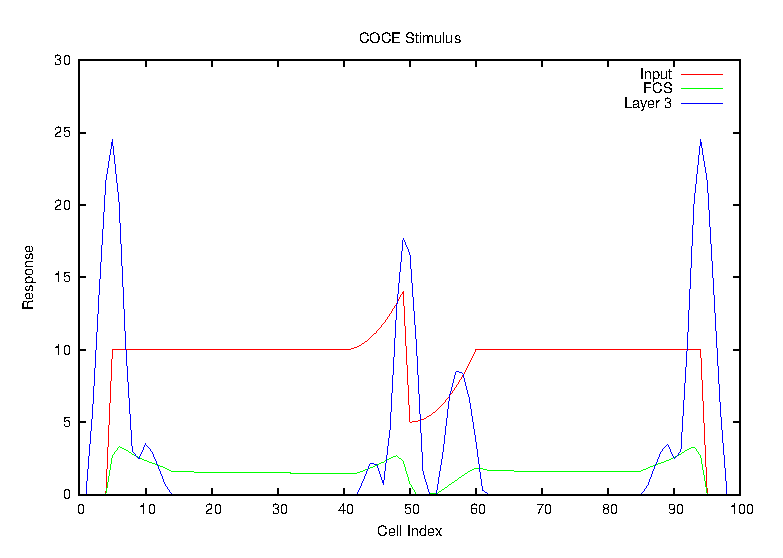
\epsfig{file=fig3.eps,width=15cm,height=11cm}
    \caption{\label{pict1}BCS and FCS output}
  \end{figure}
\end{center}

The results when presented with the non-illusory counterpart of the COCE were more indicative of those in the paper, though they were not entirely spot on. 

\begin{center}
  \begin{figure}[h!]
    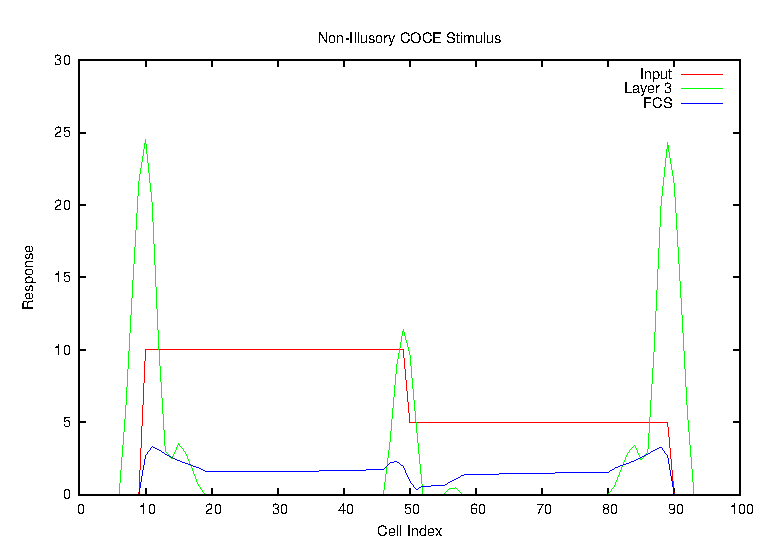
\epsfig{file=fig4.eps,width=15cm,height=11cm}
    \caption{\label{pict1}BCS and FCS output}
  \end{figure}
\end{center}

It seems to me that the major source of error were small perturbations in the BCS output that ended up signficantly impacting the FCS. Changing the parameter $L$ from 5 to 10 helped eliminate some of these, though they didn't entirely fix my problems. 

\begin{center}
  \begin{figure}[h!]
    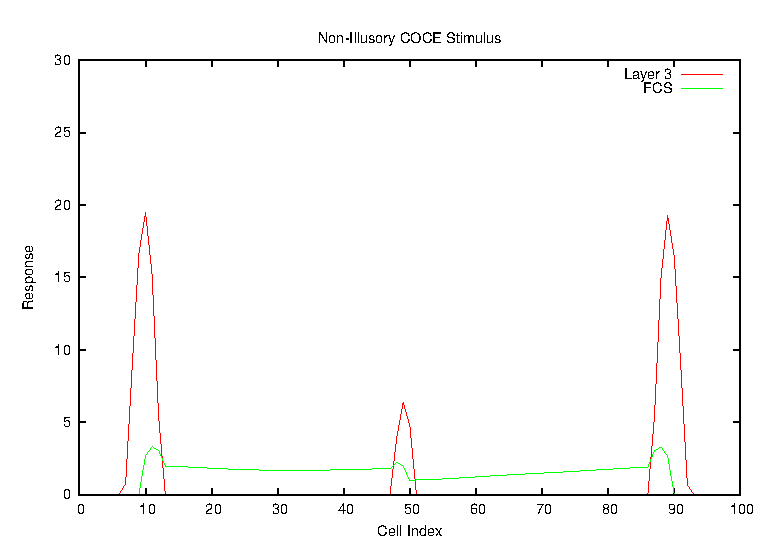
\epsfig{file=fig5.eps,width=15cm,height=11cm}
    \caption{\label{pict1}BCS and FCS output}
  \end{figure}
\end{center}

Making this change in the COCE plot did not fix things, so I bumped $L$ up to 15. 

\begin{center}
  \begin{figure}[h!]
    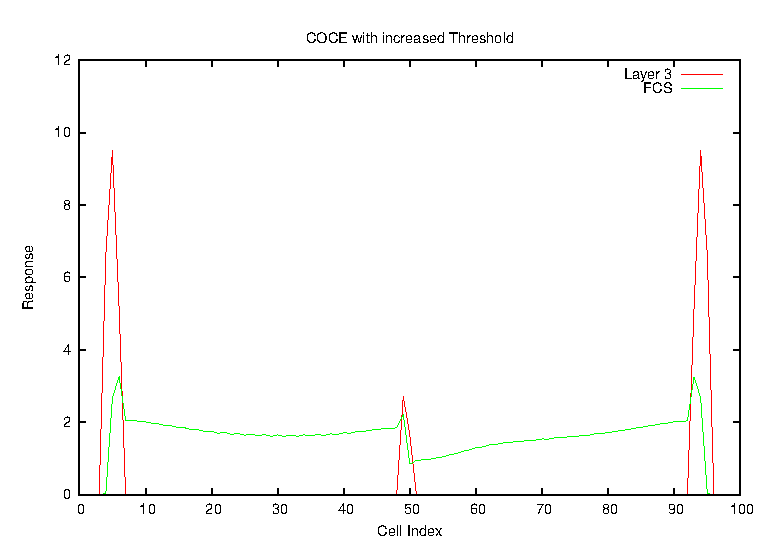
\epsfig{file=fig6.eps,width=15cm,height=11cm}
    \caption{\label{pict1}BCS and FCS output}
  \end{figure}
\end{center}

Here at least the response of the FCS between my version of the non-illusory and illusory COCE look somewhat similar, though neither are particularly indicative of the real thing. Part of this could be due to the very slow spread of input within the boundaries. Methods of solving for this will be discussed in the next section, but in terms of the parameters that govern this I got the most out of $\delta$ and $\epsilon$. Increasing $\delta$ increases the rate of diffusion, and decreasing $\epsilon$ mitigates the impact the boundaries have on the spread. I set these values to $\delta=1000$ and $\epsilon=500$, which is very different from what was suggested in the appendix. Further adjustment of these and other parameters in the FCS computation may alleviate some of my issues, but I think there is more at play that I'm not seeing. 

{\bf Convergence of Diffusion Computation}

The problem statement mentions three possible ways of solving for the diffusion equation. I chose to solve it using a relaxation method as well as a numerical simulation using the trapezoidal approximation. Neither were particularly effective, though both drastically slowed down in a similar number of steps. The error at any given iteration/time step in these methods was computed as 

\begin{equation}
e=\frac{1}{2}[\sqrt{(S[i+1]-S[i])^2}+\sqrt{(S[i-1]-S[i])^2}]
\end{equation}

\begin{center}
  \begin{figure}[h!]
    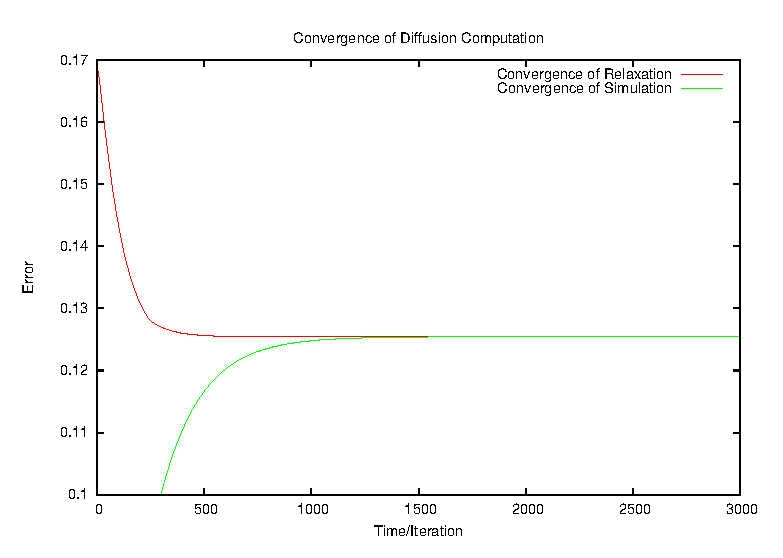
\epsfig{file=fig7.eps,width=15cm,height=11cm}
    \caption{\label{pict1}Convergence of Solving Techniques}
  \end{figure}
\end{center}

Interestingly, both converged to the same result. This can be seein in the FCS output; both yielded identical results when presented with the same parameters. This is not what I expected, but I verified it by changing the number of iteration steps in one and not the other. Both converge at roughly the same point (1000 relaxation iterations and 1000 time steps). The runtime of both methods were comparable, though I would like to try solving it using the matrix method mentioned in the problem statement. 
\smallskip

{\bf Item 2}
\smallskip

As I mentioned before, the results of Layer Six are computed by allowing the results from Layer 2 to spread within the boundaries computed by Layer 5. In order to create a ramped output in Layer 6, it follows that we should generate two boundaries in Layer 5. At one of these boundaries the response of Layer two should be larger than it is at the other boundary, and the diffusion process should result in a smooth gradient between the two. 
\smallskip

The machinery for creating a ramp exists within Layer 6, but I had trouble getting Layer 2 to have the output I desired. More often than not the results would go zero. This is because of the aspect of the distant-dependent shunting equation used to model the neurons in this layer. This equation results in a ``normalized'' input across nodes, meaning that any sort of brightness gradient gets transformed into a uniform input. 
\smallskip

It may be possible to generate a ramp with an additive equation used to model the receptive fields of layer 2. We could also allow some of the input going directly into Layer 1 to impact Layer 6 in some way in order to counteract some of these effects. The normalization and edge detection properties of Layer 2 are useful generating the data that will be used to create the BCS, but they may not be the best input to supply to Layer 6 in this case.
\smallskip

Here are some attempts of mine to generate a ramp. The first is the method of one large input at one end of the field.  

\begin{center}
  \begin{figure}[h!]
    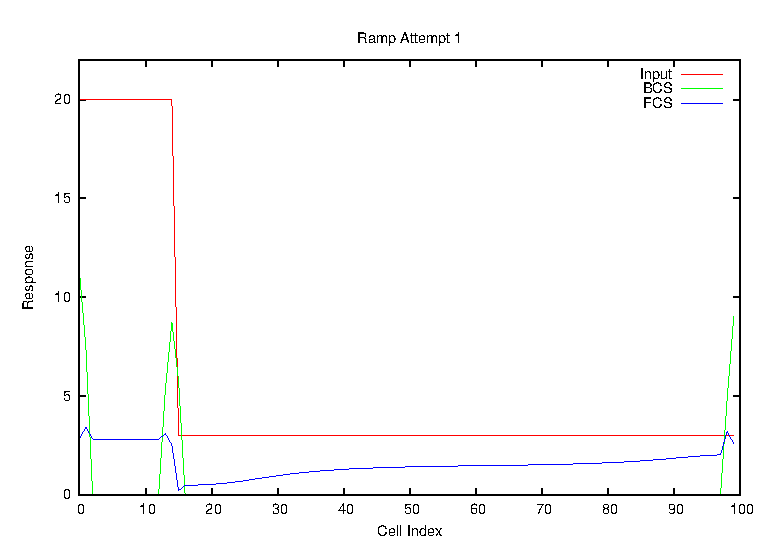
\epsfig{file=fig8.eps,width=15cm,height=11cm}
    \caption{\label{pict1}First Ramp Attempt}
  \end{figure}
\end{center}

Some semblance of a ramp can be seen there, though I attribute this to properties of my FCS in general more than anything else. I also tried an input with several intermediate stimuli, hoping the FCS would ``interpolate'' between them. 

\begin{center}
  \begin{figure}[h!]
    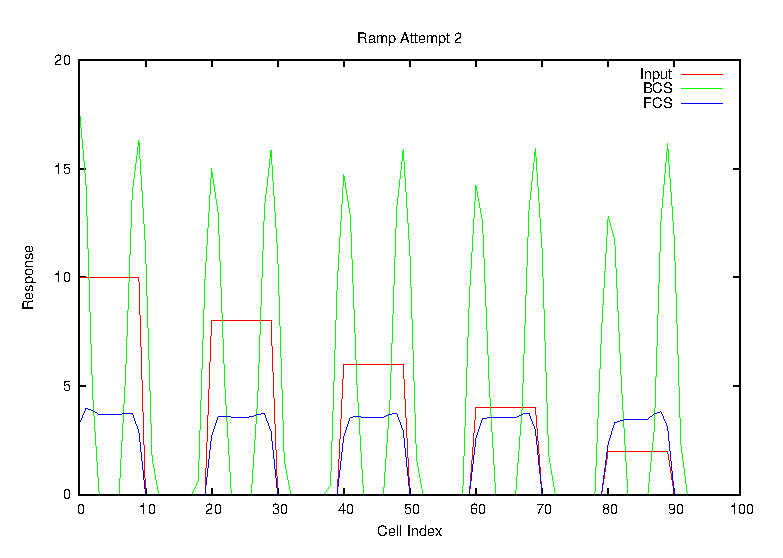
\epsfig{file=fig9.eps,width=15cm,height=11cm}
    \caption{\label{pict1}Second Ramp Attempt}
  \end{figure}
\end{center}

This one was interesting because although each bump has a different intensity, my FCS percieved them as uniform. Though there is no ramp I don't know why I expected one in the first place, and as far as things go this response seems pretty tame. 

\bigskip

{\bf Item 3}
\smallskip

My input for Item 3 consists of a 100-cell receptive field. The input of the first and last 10 nodes are 0, and every node in between has an input of 10. The 1-d projection of the half-toroidal kernel described by Craft would look as follows:

\begin{center}
  \begin{figure}[h!]
    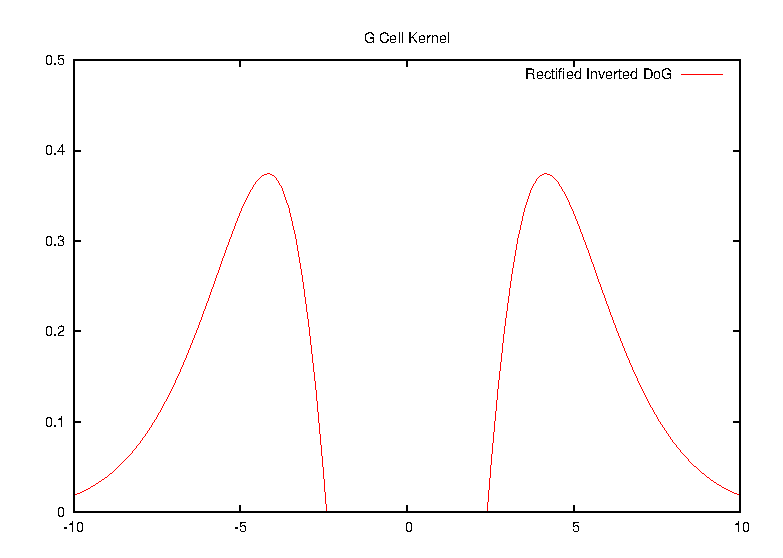
\epsfig{file=fig10.eps,width=15cm,height=11cm}
    \caption{\label{pict1}Rectified Inverted DoG Kernel}
  \end{figure}
\end{center}

It is essentially the two outer bumps of the DoG kernel. The left bump and right bump form the two fragmented kernels mentioned in the assignment. The equation for this kernel and its two zeroes:

\begin{equation}

\end{eqnarray}
G(x)=-(Ae^{(\frac{x}{b})^2}-Ce^{(\frac{x}{d})^2}) \\
x_z=\pm \frac{(b*d*\sqrt{ln(\frac{A}{C})})}{\sqrt{d^2-b^2} 
\end{eqnarray}

In order to convolve a field with the left or right input, we start at either the left or right zero and move outward using the equation described above. 
\smallskip

To numerically integrate these equations I will be using the Rotter-Deismann method (the equations are linear, so this seems Kosher.) I found that the results from either $B$ cell were nearly indistinguishable, though their modulation index did contain some information. In this graph only the left cell output is plotted alongside the G cell output. The input provided was a simple bar input. 

\begin{center}
  \begin{figure}[h!]
    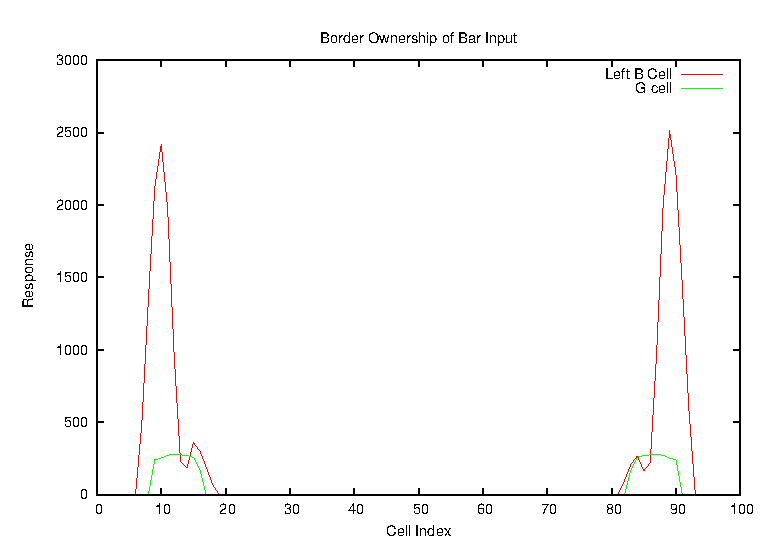
\epsfig{file=fig11.eps,width=15cm,height=11cm}
    \caption{\label{pict1}Rectified Inverted DoG Kernel}
  \end{figure}
\end{center}

Notice that these response values are much larger than anything seen before. The modulation index for this bar input looks like this:

\begin{center}
  \begin{figure}[h!]
    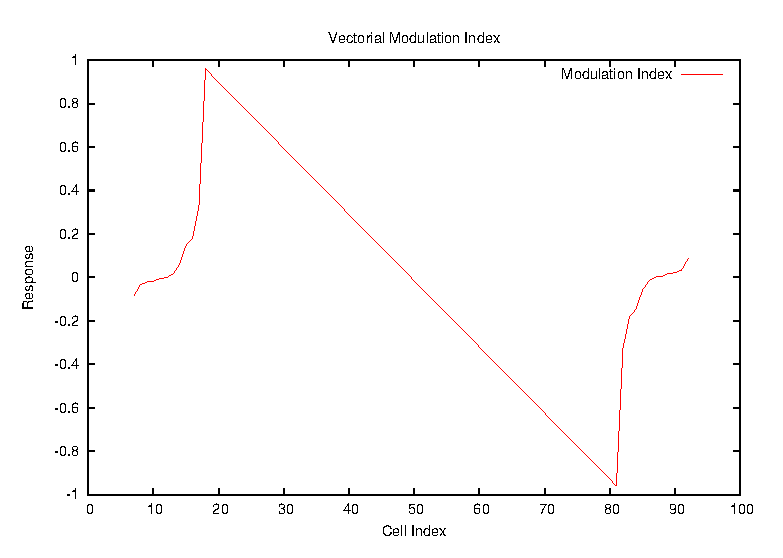
\epsfig{file=fig12.eps,width=15cm,height=11cm}
    \caption{\label{pict1}Rectified Inverted DoG Kernel}
  \end{figure}
\end{center}

These values are normalized between -1 and 1 by the nature of the equation, and show that border ownership is given to the bar in the middle. 
\smallskip

In the G cell equation the left and right cell responses are summed together in order to compute the magnitude, or total border ownership, in this region of the field. A generalization of this in 2-D would be finding the magnitude of edges going up, down, left or right. 
\smallskip

I'm not entirely sure what Group cells are meant to represent, but in my model (which may be incorrect) they fire given the presence of a border, implying they can be used to segment an image into regions of different groups. This differs from what the BCS does because of the left-right convolutions, meaning the term under the radical in the G equation fires only in the presence of spatially directed changes in stimuli. 
\smallskip

An input that seemed to have some trouble was the second one I used when trying to generate a ramp in Item 2. I call this input the Stepping Stone Input. 

\begin{center}
  \begin{figure}[h!]
    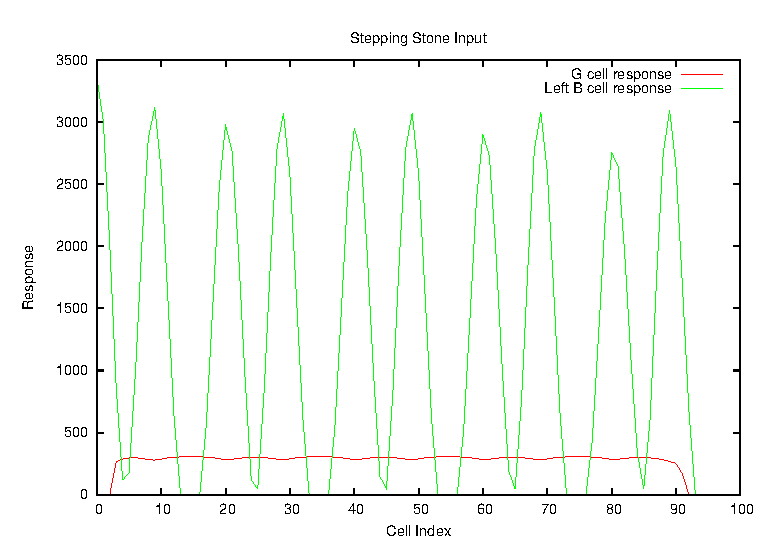
\epsfig{file=fig13.eps,width=15cm,height=11cm}
    \caption{\label{pict1}Rectified Inverted DoG Kernel}
  \end{figure}
\end{center}

It could be that the borders were too close and got muddled in between each other, hence the single G cell response encompassing the whole region. The vectorial modulation index is what we'd expect, which is to say it is not very interesting. 

\begin{center}
  \begin{figure}[h!]
    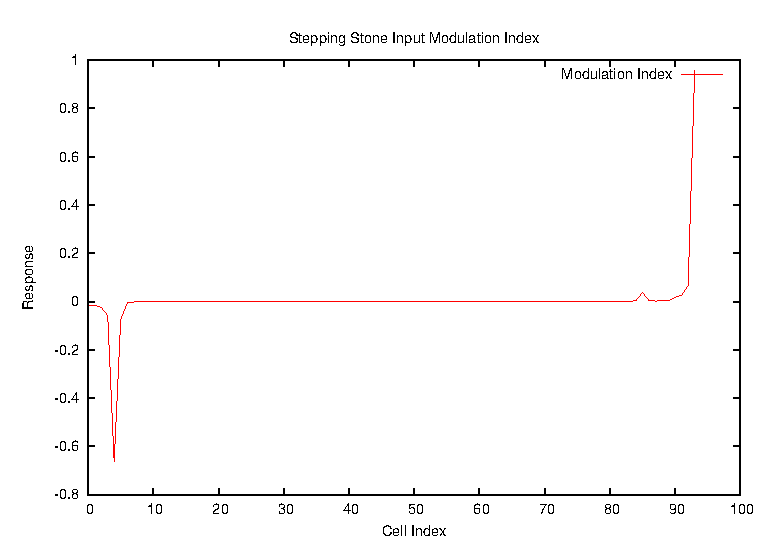
\epsfig{file=fig14.eps,width=15cm,height=11cm}
    \caption{\label{pict1}Rectified Inverted DoG Kernel}
  \end{figure}
\end{center}

I'm not really sure what the comparison to the FCS/BCS system is here, since this model essentially uses the BCS and generates something that appears to be different. Maybe the similarity is that it uses these boundaries, but it seems to me that the models have different goals in mind. 

\end{document}
